\documentclass{beamer}
\usetheme{default}
\usecolortheme{default}

%% custom color theme. 
\definecolor{sidebartop}{RGB}{133,135,86}
\definecolor{sidebar}{RGB}{177,179,115}
\definecolor{sidebarbot}{RGB}{211,213,136}
\definecolor{title}{RGB}{241,243,186}
\setbeamertemplate{sidebar canvas left}[vertical shading][top=sidebar,bottom=sidebarbot]
\setbeamercolor{frametitle}{fg=title,bg=sidebar}
\setbeamercolor{logo}{fg=sidebar,bg=sidebar}
\setbeamercolor{sidebar}{fg=sidebarbot}
\setbeamercolor{title in sidebar}{fg=title}
\setbeamercolor{author in sidebar}{fg=title}
\setbeamercolor{section in sidebar}{fg=white}
\setbeamercolor{section in sidebar shaded}{fg=title}
\setbeamercolor{item}{fg=sidebar}

%%%%%%%%%%%%%%%%%%
%% For printing handout
%\documentclass[handout]{beamer}
%\usepackage{pgfpages}
%\pgfpagesuselayout{2 on 1}[letterpaper,border shrink=10mm]
%%\pgfpageslogicalpageoptions{1}{border code=\pgfusepath{stroke}}
%%\pgfpageslogicalpageoptions{2}{border code=\pgfusepath{stroke}}
%\usetheme{default}
%\usecolortheme{default}
%% Handout commands end here
%%%%%%%%%%%%%%%%%%

\usepackage{color}
\usepackage{graphicx}

\usepackage[lined]{algorithm2e}

%\usepackage{bibentry}
%\nobibliography*
\begin{document}
{
\usebackgroundtemplate{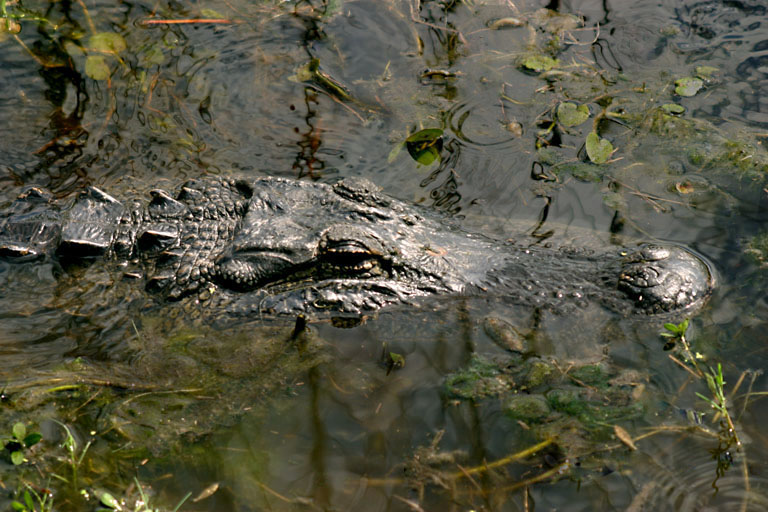
\includegraphics[height=\paperheight]{figure/GatorHeadModified.jpg}}
\begin{frame}[plain,c]
% \vspace*{-0.1in}
\begin{center}
  {\color[RGB]{241,243,186}
{\huge EEL6935 Course Project Proposal\\
    \vspace*{0.5em}
    Sentence Classification Using a CNN}\\
  \vspace*{1.8in}
    Caleb Bryent, {\bf Jixin Feng}, Hao Huang \\
    \vspace*{1em}
  \begin{tabular}{cc}
  University of Florida
   \end{tabular}
}
  \end{center}
\hoffset=0em
\end{frame}}

\begin{frame}
\frametitle{Background}
    \begin{columns}
    \begin{column}{0.5\textwidth}
    \begin{itemize}
        \item Tremendous volume of unstructured text generated everyday
        \item 40ZB ($40\times 10^{21}$bytes) by year 2020, 50-fold from 2010\footnotemark
        \item generated from news media, social networks, medical records, 
            business transactions\ldots
        \item effective processing method is needed
    \end{itemize}
    \end{column}
    \begin{column}{0.5\textwidth}
    \center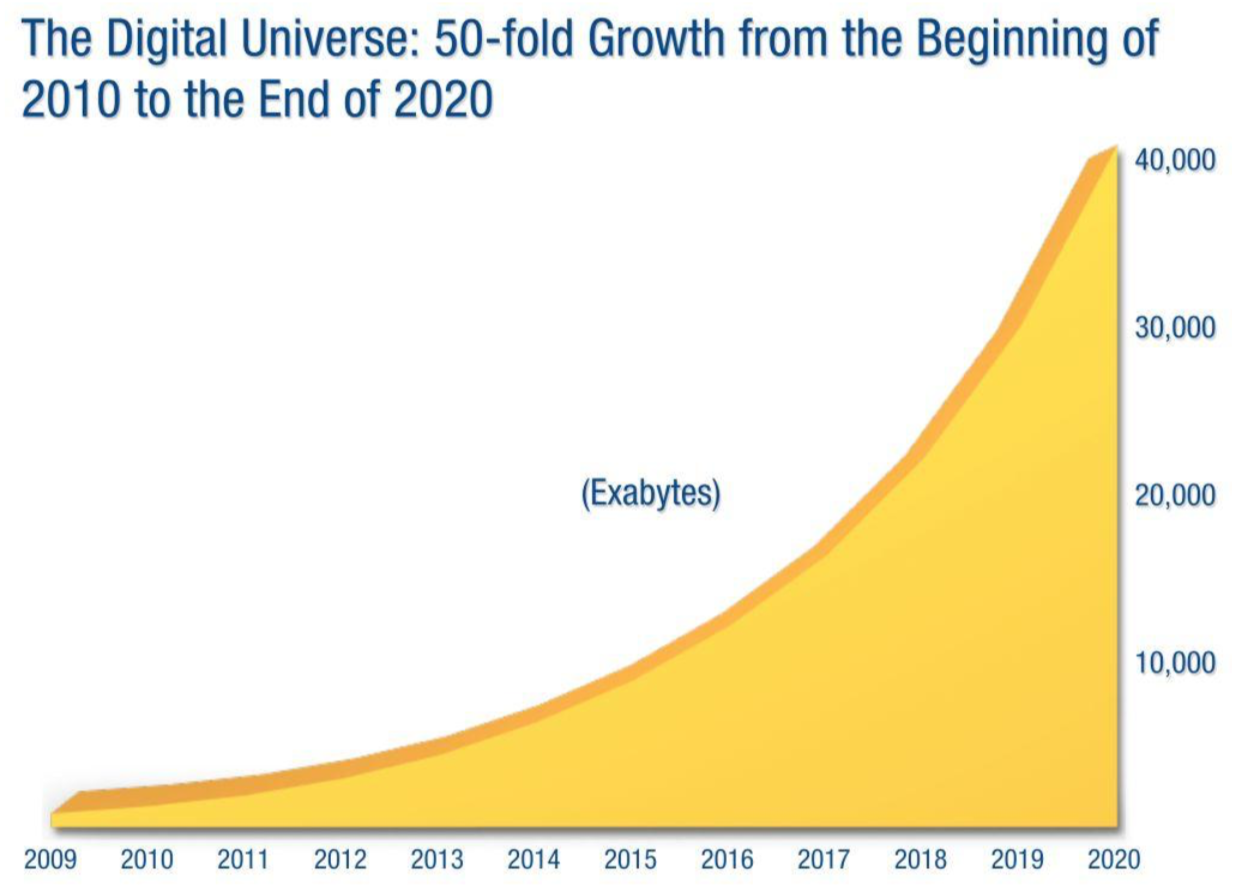
\includegraphics[width=\textwidth]{figure/data_growth_2020}
    \end{column}
    \end{columns}
    \footnotetext[1]{Gantz, J., \& Reinsel, D. (2012). The digital universe in 2020: Big data, bigger digital shadows, and biggest growth in the far east. IDC iView: IDC Analyze the future, 2007(2012), 1-16.}
\end{frame}

\begin{frame}
\frametitle{Sentence Classification}
    Goal: assign pre-defined labels to a sentence, categorize topic.
    $$f:\mathcal{D}\rightarrow\mathcal{L}$$
    \begin{itemize}
        \item $\mathcal{D}=\{d_0, d_1,\ldots, d_{n-1}\}$ is the set of sentence
        \item $\mathcal{L}=\{l_0, l_1,\ldots, l_{k-1}\}$ is the set of labels.
    \end{itemize}
    The performance can be measured by $F_1$ Score:
    $$F_1=\frac{2}{\frac{1}{r}+\frac{1}{p}}=\frac{2pr}{p+r}$$
    \begin{itemize}
        \item Precision: $p=\frac{tpr}{tpr+fpr}$
        \item Recall: $r=\frac{tpr}{tpr+fnr}$
    \end{itemize}
\end{frame}

\begin{frame}
\frametitle{Sentence Classification by CNN}
        \begin{columns}
    \begin{column}{0.5\textwidth}
    \center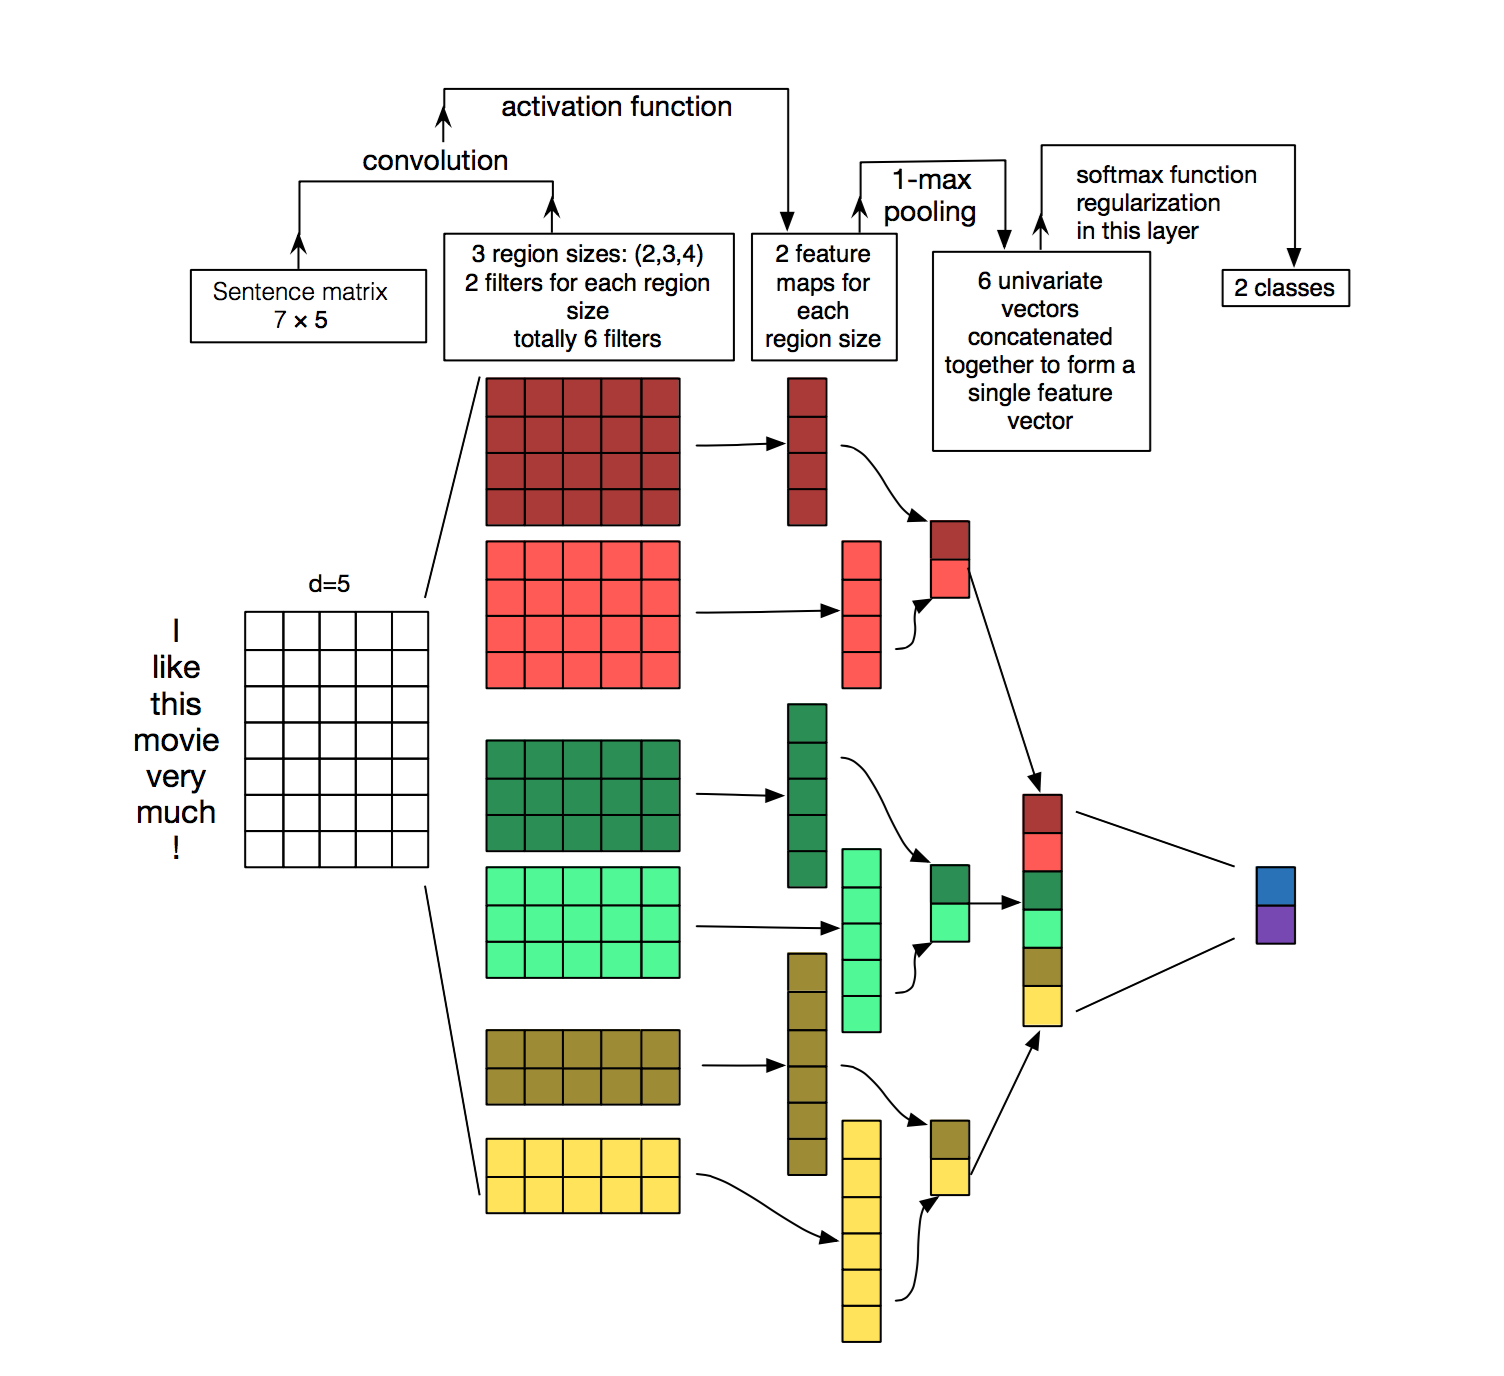
\includegraphics[width=\textwidth]{figure/sc_cnn}
    \end{column}
    \begin{column}{0.5\textwidth}
    \begin{itemize}
        \item Historically via naive Bayes, nearest neighbor, decision trees, SVM, etc.
        \item Propose to implement a sentence classifier based on CNN
        \item CNN originally designed for computer vision
        \item Shown significant potential in NLP
    \end{itemize}
    \end{column}
    \end{columns}
    \footnotetext{Plot credit: http://www.wildml.com/2015/11/understanding-convolutional-neural-networks-for-nlp/}
\end{frame}

\begin{frame}
\frametitle{System Model}
    
\end{frame}

\begin{frame}
\center{\huge Thank You!}
\center Questions?
\end{frame}
\end{document}
